\documentclass[1p]{elsarticle_modified}
%\bibliographystyle{elsarticle-num}

%\usepackage[colorlinks]{hyperref}
%\usepackage{abbrmath_seonhwa} %\Abb, \Ascr, \Acal ,\Abf, \Afrak
\usepackage{amsfonts}
\usepackage{amssymb}
\usepackage{amsmath}
\usepackage{amsthm}
\usepackage{scalefnt}
\usepackage{amsbsy}
\usepackage{kotex}
\usepackage{caption}
\usepackage{subfig}
\usepackage{color}
\usepackage{graphicx}
\usepackage{xcolor} %% white, black, red, green, blue, cyan, magenta, yellow
\usepackage{float}
\usepackage{setspace}
\usepackage{hyperref}

\usepackage{tikz}
\usetikzlibrary{arrows}

\usepackage{multirow}
\usepackage{array} % fixed length table
\usepackage{hhline}

%%%%%%%%%%%%%%%%%%%%%
\makeatletter
\renewcommand*\env@matrix[1][\arraystretch]{%
	\edef\arraystretch{#1}%
	\hskip -\arraycolsep
	\let\@ifnextchar\new@ifnextchar
	\array{*\c@MaxMatrixCols c}}
\makeatother %https://tex.stackexchange.com/questions/14071/how-can-i-increase-the-line-spacing-in-a-matrix
%%%%%%%%%%%%%%%

\usepackage[normalem]{ulem}

\newcommand{\msout}[1]{\ifmmode\text{\sout{\ensuremath{#1}}}\else\sout{#1}\fi}
%SOURCE: \msout is \stkout macro in https://tex.stackexchange.com/questions/20609/strikeout-in-math-mode

\newcommand{\cancel}[1]{
	\ifmmode
	{\color{red}\msout{#1}}
	\else
	{\color{red}\sout{#1}}
	\fi
}

\newcommand{\add}[1]{
	{\color{blue}\uwave{#1}}
}

\newcommand{\replace}[2]{
	\ifmmode
	{\color{red}\msout{#1}}{\color{blue}\uwave{#2}}
	\else
	{\color{red}\sout{#1}}{\color{blue}\uwave{#2}}
	\fi
}

\newcommand{\Sol}{\mathcal{S}} %segment
\newcommand{\D}{D} %diagram
\newcommand{\A}{\mathcal{A}} %arc


%%%%%%%%%%%%%%%%%%%%%%%%%%%%%5 test

\def\sl{\operatorname{\textup{SL}}(2,\Cbb)}
\def\psl{\operatorname{\textup{PSL}}(2,\Cbb)}
\def\quan{\mkern 1mu \triangleright \mkern 1mu}

\theoremstyle{definition}
\newtheorem{thm}{Theorem}[section]
\newtheorem{prop}[thm]{Proposition}
\newtheorem{lem}[thm]{Lemma}
\newtheorem{ques}[thm]{Question}
\newtheorem{cor}[thm]{Corollary}
\newtheorem{defn}[thm]{Definition}
\newtheorem{exam}[thm]{Example}
\newtheorem{rmk}[thm]{Remark}
\newtheorem{alg}[thm]{Algorithm}

\newcommand{\I}{\sqrt{-1}}
\begin{document}

%\begin{frontmatter}
%
%\title{Boundary parabolic representations of knots up to 8 crossings}
%
%%% Group authors per affiliation:
%\author{Yunhi Cho} 
%\address{Department of Mathematics, University of Seoul, Seoul, Korea}
%\ead{yhcho@uos.ac.kr}
%
%
%\author{Seonhwa Kim} %\fnref{s_kim}}
%\address{Center for Geometry and Physics, Institute for Basic Science, Pohang, 37673, Korea}
%\ead{ryeona17@ibs.re.kr}
%
%\author{Hyuk Kim}
%\address{Department of Mathematical Sciences, Seoul National University, Seoul 08826, Korea}
%\ead{hyukkim@snu.ac.kr}
%
%\author{Seokbeom Yoon}
%\address{Department of Mathematical Sciences, Seoul National University, Seoul, 08826,  Korea}
%\ead{sbyoon15@snu.ac.kr}
%
%\begin{abstract}
%We find all boundary parabolic representation of knots up to 8 crossings.
%
%\end{abstract}
%\begin{keyword}
%    \MSC[2010] 57M25 
%\end{keyword}
%
%\end{frontmatter}

%\linenumbers
%\tableofcontents
%
\newcommand\colored[1]{\textcolor{white}{\rule[-0.35ex]{0.8em}{1.4ex}}\kern-0.8em\color{red} #1}%
%\newcommand\colored[1]{\textcolor{white}{ #1}\kern-2.17ex	\textcolor{white}{ #1}\kern-1.81ex	\textcolor{white}{ #1}\kern-2.15ex\color{red}#1	}

{\Large $\underline{12a_{0225}~(K12a_{0225})}$}

\setlength{\tabcolsep}{10pt}
\renewcommand{\arraystretch}{1.6}
\vspace{1cm}\begin{tabular}{m{100pt}>{\centering\arraybackslash}m{274pt}}
\multirow{5}{120pt}{
	\centering
	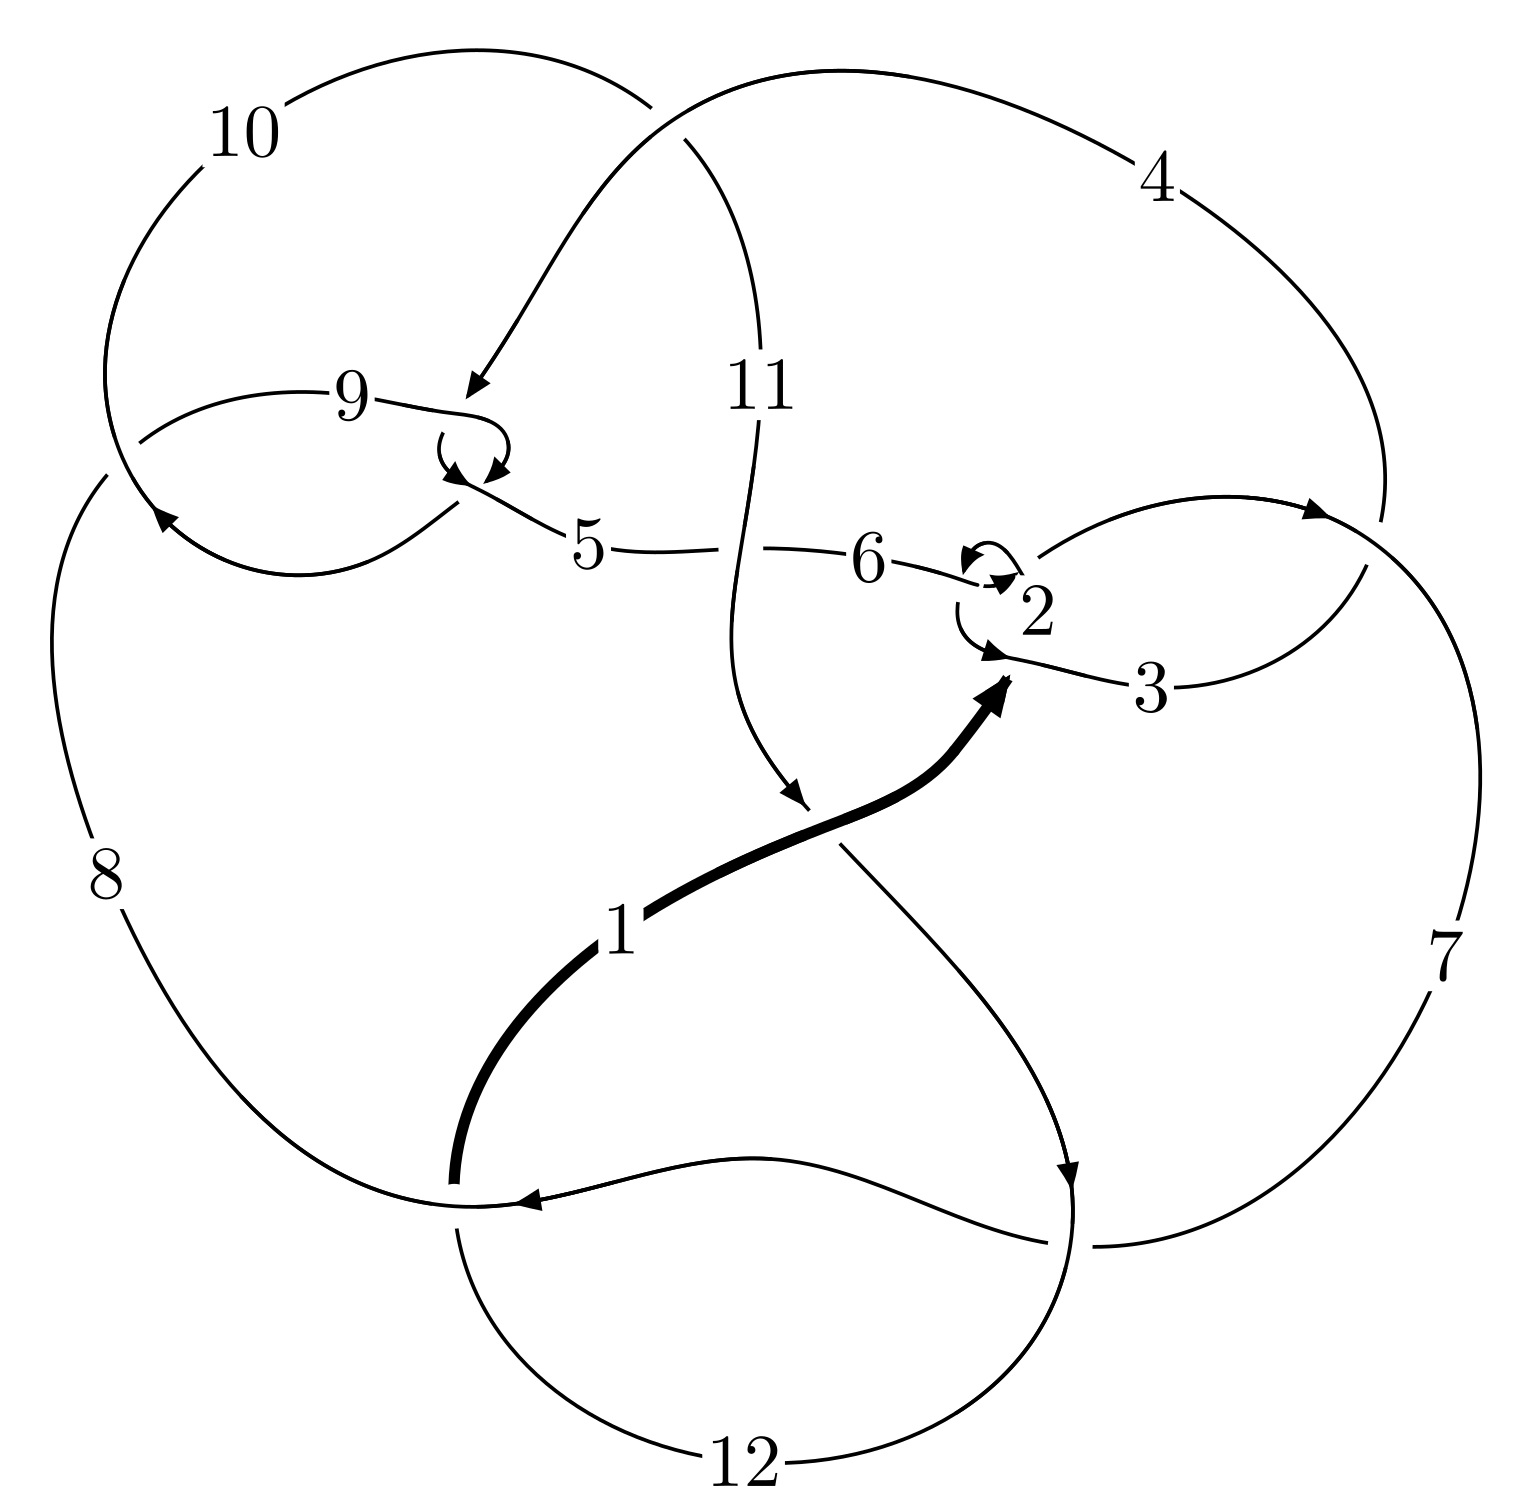
\includegraphics[width=112pt]{../../../GIT/diagram.site/Diagrams/png/1026_12a_0225.png}\\
\ \ \ A knot diagram\footnotemark}&
\allowdisplaybreaks
\textbf{Linearized knot diagam} \\
\cline{2-2}
 &
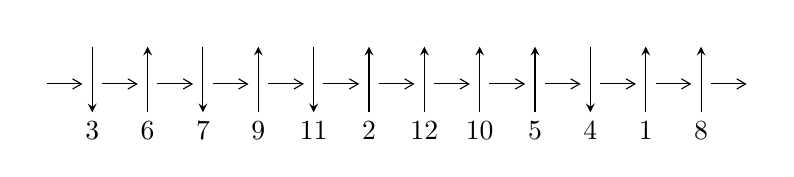
\begin{tikzpicture}[x=20pt, y=17pt]
	% nodes
	\node (C0) at (0, 0) {};
	\node (C1) at (1, 0) {};
	\node (C1U) at (1, +1) {};
	\node (C1D) at (1, -1) {3};

	\node (C2) at (2, 0) {};
	\node (C2U) at (2, +1) {};
	\node (C2D) at (2, -1) {6};

	\node (C3) at (3, 0) {};
	\node (C3U) at (3, +1) {};
	\node (C3D) at (3, -1) {7};

	\node (C4) at (4, 0) {};
	\node (C4U) at (4, +1) {};
	\node (C4D) at (4, -1) {9};

	\node (C5) at (5, 0) {};
	\node (C5U) at (5, +1) {};
	\node (C5D) at (5, -1) {11};

	\node (C6) at (6, 0) {};
	\node (C6U) at (6, +1) {};
	\node (C6D) at (6, -1) {2};

	\node (C7) at (7, 0) {};
	\node (C7U) at (7, +1) {};
	\node (C7D) at (7, -1) {12};

	\node (C8) at (8, 0) {};
	\node (C8U) at (8, +1) {};
	\node (C8D) at (8, -1) {10};

	\node (C9) at (9, 0) {};
	\node (C9U) at (9, +1) {};
	\node (C9D) at (9, -1) {5};

	\node (C10) at (10, 0) {};
	\node (C10U) at (10, +1) {};
	\node (C10D) at (10, -1) {4};

	\node (C11) at (11, 0) {};
	\node (C11U) at (11, +1) {};
	\node (C11D) at (11, -1) {1};

	\node (C12) at (12, 0) {};
	\node (C12U) at (12, +1) {};
	\node (C12D) at (12, -1) {8};
	\node (C13) at (13, 0) {};

	% arrows
	\draw[->,>={angle 60}]
	(C0) edge (C1) (C1) edge (C2) (C2) edge (C3) (C3) edge (C4) (C4) edge (C5) (C5) edge (C6) (C6) edge (C7) (C7) edge (C8) (C8) edge (C9) (C9) edge (C10) (C10) edge (C11) (C11) edge (C12) (C12) edge (C13) ;	\draw[->,>=stealth]
	(C1U) edge (C1D) (C2D) edge (C2U) (C3U) edge (C3D) (C4D) edge (C4U) (C5U) edge (C5D) (C6D) edge (C6U) (C7D) edge (C7U) (C8D) edge (C8U) (C9D) edge (C9U) (C10U) edge (C10D) (C11D) edge (C11U) (C12D) edge (C12U) ;
	\end{tikzpicture} \\
\hhline{~~} \\& 
\textbf{Solving Sequence} \\ \cline{2-2} 
 &
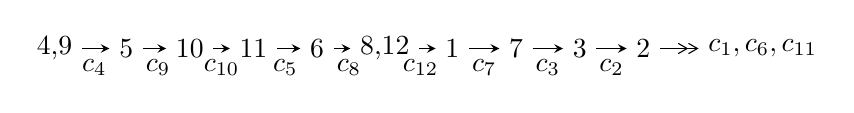
\begin{tikzpicture}[x=23pt, y=7pt]
	% node
	\node (A0) at (-1/8, 0) {4,9};
	\node (A1) at (1, 0) {5};
	\node (A2) at (2, 0) {10};
	\node (A3) at (3, 0) {11};
	\node (A4) at (4, 0) {6};
	\node (A5) at (81/16, 0) {8,12};
	\node (A6) at (49/8, 0) {1};
	\node (A7) at (57/8, 0) {7};
	\node (A8) at (65/8, 0) {3};
	\node (A9) at (73/8, 0) {2};
	\node (C1) at (1/2, -1) {$c_{4}$};
	\node (C2) at (3/2, -1) {$c_{9}$};
	\node (C3) at (5/2, -1) {$c_{10}$};
	\node (C4) at (7/2, -1) {$c_{5}$};
	\node (C5) at (9/2, -1) {$c_{8}$};
	\node (C6) at (45/8, -1) {$c_{12}$};
	\node (C7) at (53/8, -1) {$c_{7}$};
	\node (C8) at (61/8, -1) {$c_{3}$};
	\node (C9) at (69/8, -1) {$c_{2}$};
	\node (A10) at (11, 0) {$c_{1},c_{6},c_{11}$};

	% edge
	\draw[->,>=stealth]	
	(A0) edge (A1) (A1) edge (A2) (A2) edge (A3) (A3) edge (A4) (A4) edge (A5) (A5) edge (A6) (A6) edge (A7) (A7) edge (A8) (A8) edge (A9) ;
	\draw[->>,>={angle 60}]	
	(A9) edge (A10);
\end{tikzpicture} \\ 

\end{tabular} \\

\footnotetext{
The image of knot diagram is generated by the software ``\textbf{Draw programme}" developed by Andrew Bartholomew(\url{http://www.layer8.co.uk/maths/draw/index.htm\#Running-draw}), where we modified some parts for our purpose(\url{https://github.com/CATsTAILs/LinksPainter}).
}\phantom \\ \newline 
\centering \textbf{Ideals for irreducible components\footnotemark of $X_{\text{par}}$} 
 
\begin{align*}
I^u_{1}&=\langle 
4.07777\times10^{66} u^{126}+2.16707\times10^{66} u^{125}+\cdots+1.72852\times10^{66} b-4.32805\times10^{66},\\
\phantom{I^u_{1}}&\phantom{= \langle  }7.32061\times10^{65} u^{126}-1.66742\times10^{66} u^{125}+\cdots+1.72852\times10^{66} a-1.52406\times10^{67},\;u^{127}+u^{126}+\cdots-4 u-4\rangle \\
I^u_{2}&=\langle 
u^2 a- u^3+2 b+u,\;-6 u^3 a+2 u^2 a+2 a^2+5 u^2-4 a+6 u-14,\;u^4-2 u^2+2\rangle \\
\\
I^v_{1}&=\langle 
a,\;b- v+1,\;v^2- v+1\rangle \\
\end{align*}
\raggedright * 3 irreducible components of $\dim_{\mathbb{C}}=0$, with total 137 representations.\\
\footnotetext{All coefficients of polynomials are rational numbers. But the coefficients are sometimes approximated in decimal forms when there is not enough margin.}
\newpage
\renewcommand{\arraystretch}{1}
\centering \section*{I. $I^u_{1}= \langle 4.08\times10^{66} u^{126}+2.17\times10^{66} u^{125}+\cdots+1.73\times10^{66} b-4.33\times10^{66},\;7.32\times10^{65} u^{126}-1.67\times10^{66} u^{125}+\cdots+1.73\times10^{66} a-1.52\times10^{67},\;u^{127}+u^{126}+\cdots-4 u-4 \rangle$}
\flushleft \textbf{(i) Arc colorings}\\
\begin{tabular}{m{7pt} m{180pt} m{7pt} m{180pt} }
\flushright $a_{4}=$&$\begin{pmatrix}1\\0\end{pmatrix}$ \\
\flushright $a_{9}=$&$\begin{pmatrix}0\\u\end{pmatrix}$ \\
\flushright $a_{5}=$&$\begin{pmatrix}1\\- u^2\end{pmatrix}$ \\
\flushright $a_{10}=$&$\begin{pmatrix}u\\- u^3+u\end{pmatrix}$ \\
\flushright $a_{11}=$&$\begin{pmatrix}u^3\\- u^3+u\end{pmatrix}$ \\
\flushright $a_{6}=$&$\begin{pmatrix}u^8- u^6+u^4+1\\- u^8+2 u^6-2 u^4\end{pmatrix}$ \\
\flushright $a_{8}=$&$\begin{pmatrix}- u^3\\u^5- u^3+u\end{pmatrix}$ \\
\flushright $a_{12}=$&$\begin{pmatrix}-0.423519 u^{126}+0.964650 u^{125}+\cdots+9.44857 u+8.81712\\-2.35911 u^{126}-1.25371 u^{125}+\cdots+6.16306 u+2.50390\end{pmatrix}$ \\
\flushright $a_{1}=$&$\begin{pmatrix}-0.00503774 u^{126}+0.683855 u^{125}+\cdots+7.43488 u+5.05619\\-1.38708 u^{126}-0.530217 u^{125}+\cdots+5.40266 u+1.20161\end{pmatrix}$ \\
\flushright $a_{7}=$&$\begin{pmatrix}-0.189021 u^{126}-0.0433393 u^{125}+\cdots-5.68886 u-0.558061\\-0.137798 u^{126}+0.166256 u^{125}+\cdots+3.26326 u-0.549191\end{pmatrix}$ \\
\flushright $a_{3}=$&$\begin{pmatrix}-0.406855 u^{126}+0.266501 u^{125}+\cdots+5.53868 u+7.25484\\-3.21774 u^{126}-1.72302 u^{125}+\cdots+6.64167 u+4.67939\end{pmatrix}$ \\
\flushright $a_{2}=$&$\begin{pmatrix}-0.202280 u^{126}-0.184206 u^{125}+\cdots+3.16129 u+3.06932\\-2.22568 u^{126}-1.02528 u^{125}+\cdots+5.29101 u+3.62099\end{pmatrix}$\\&\end{tabular}
\flushleft \textbf{(ii) Obstruction class $= -1$}\\~\\
\flushleft \textbf{(iii) Cusp Shapes $= 2.57051 u^{126}+2.63831 u^{125}+\cdots+11.3436 u+1.19661$}\\~\\
\newpage\renewcommand{\arraystretch}{1}
\flushleft \textbf{(iv) u-Polynomials at the component}\newline \\
\begin{tabular}{m{50pt}|m{274pt}}
Crossings & \hspace{64pt}u-Polynomials at each crossing \\
\hline $$\begin{aligned}c_{1}\end{aligned}$$&$\begin{aligned}
&u^{127}+62 u^{126}+\cdots-34 u-25
\end{aligned}$\\
\hline $$\begin{aligned}c_{2},c_{6}\end{aligned}$$&$\begin{aligned}
&u^{127}-2 u^{126}+\cdots+24 u-5
\end{aligned}$\\
\hline $$\begin{aligned}c_{3}\end{aligned}$$&$\begin{aligned}
&u^{127}+2 u^{126}+\cdots-4532584 u-667745
\end{aligned}$\\
\hline $$\begin{aligned}c_{4},c_{9}\end{aligned}$$&$\begin{aligned}
&u^{127}+u^{126}+\cdots-4 u-4
\end{aligned}$\\
\hline $$\begin{aligned}c_{5}\end{aligned}$$&$\begin{aligned}
&u^{127}- u^{126}+\cdots-7705060 u-2511892
\end{aligned}$\\
\hline $$\begin{aligned}c_{7},c_{12}\end{aligned}$$&$\begin{aligned}
&u^{127}-3 u^{126}+\cdots+11 u-1
\end{aligned}$\\
\hline $$\begin{aligned}c_{8}\end{aligned}$$&$\begin{aligned}
&u^{127}-61 u^{126}+\cdots+80 u-16
\end{aligned}$\\
\hline $$\begin{aligned}c_{10}\end{aligned}$$&$\begin{aligned}
&u^{127}+3 u^{126}+\cdots+54716 u-9292
\end{aligned}$\\
\hline $$\begin{aligned}c_{11}\end{aligned}$$&$\begin{aligned}
&u^{127}-63 u^{126}+\cdots-9 u-1
\end{aligned}$\\
\hline
\end{tabular}\\~\\
\newpage\renewcommand{\arraystretch}{1}
\flushleft \textbf{(v) Riley Polynomials at the component}\newline \\
\begin{tabular}{m{50pt}|m{274pt}}
Crossings & \hspace{64pt}Riley Polynomials at each crossing \\
\hline $$\begin{aligned}c_{1}\end{aligned}$$&$\begin{aligned}
&y^{127}+14 y^{126}+\cdots+23706 y-625
\end{aligned}$\\
\hline $$\begin{aligned}c_{2},c_{6}\end{aligned}$$&$\begin{aligned}
&y^{127}+62 y^{126}+\cdots-34 y-25
\end{aligned}$\\
\hline $$\begin{aligned}c_{3}\end{aligned}$$&$\begin{aligned}
&y^{127}-34 y^{126}+\cdots+8331046653166 y-445883385025
\end{aligned}$\\
\hline $$\begin{aligned}c_{4},c_{9}\end{aligned}$$&$\begin{aligned}
&y^{127}-61 y^{126}+\cdots+80 y-16
\end{aligned}$\\
\hline $$\begin{aligned}c_{5}\end{aligned}$$&$\begin{aligned}
&y^{127}-29 y^{126}+\cdots+382290475250896 y-6309601419664
\end{aligned}$\\
\hline $$\begin{aligned}c_{7},c_{12}\end{aligned}$$&$\begin{aligned}
&y^{127}-63 y^{126}+\cdots-9 y-1
\end{aligned}$\\
\hline $$\begin{aligned}c_{8}\end{aligned}$$&$\begin{aligned}
&y^{127}+15 y^{126}+\cdots-5888 y-256
\end{aligned}$\\
\hline $$\begin{aligned}c_{10}\end{aligned}$$&$\begin{aligned}
&y^{127}+31 y^{126}+\cdots-5880391024 y-86341264
\end{aligned}$\\
\hline $$\begin{aligned}c_{11}\end{aligned}$$&$\begin{aligned}
&y^{127}+17 y^{126}+\cdots-473 y-1
\end{aligned}$\\
\hline
\end{tabular}\\~\\
\newpage\flushleft \textbf{(vi) Complex Volumes and Cusp Shapes}
$$\begin{array}{c|c|c}  
\text{Solutions to }I^u_{1}& \I (\text{vol} + \sqrt{-1}CS) & \text{Cusp shape}\\
 \hline 
\begin{aligned}
u &= -0.655892 + 0.693362 I \\
a &= \phantom{-}1.314510 + 0.510372 I \\
b &= \phantom{-}1.08376 + 1.72394 I\end{aligned}
 & -4.37389 - 10.57070 I & \phantom{-0.000000 } 0 \\ \hline\begin{aligned}
u &= -0.655892 - 0.693362 I \\
a &= \phantom{-}1.314510 - 0.510372 I \\
b &= \phantom{-}1.08376 - 1.72394 I\end{aligned}
 & -4.37389 + 10.57070 I & \phantom{-0.000000 } 0 \\ \hline\begin{aligned}
u &= -1.047020 + 0.069569 I \\
a &= -0.051726 + 0.443444 I \\
b &= -0.550463 + 0.034451 I\end{aligned}
 & -1.72547 - 2.55576 I & \phantom{-0.000000 } 0 \\ \hline\begin{aligned}
u &= -1.047020 - 0.069569 I \\
a &= -0.051726 - 0.443444 I \\
b &= -0.550463 - 0.034451 I\end{aligned}
 & -1.72547 + 2.55576 I & \phantom{-0.000000 } 0 \\ \hline\begin{aligned}
u &= \phantom{-}0.634680 + 0.668715 I \\
a &= -1.136010 + 0.469975 I \\
b &= -0.91228 + 1.61811 I\end{aligned}
 & -1.74528 + 5.54287 I & \phantom{-0.000000 } 0 \\ \hline\begin{aligned}
u &= \phantom{-}0.634680 - 0.668715 I \\
a &= -1.136010 - 0.469975 I \\
b &= -0.91228 - 1.61811 I\end{aligned}
 & -1.74528 - 5.54287 I & \phantom{-0.000000 } 0 \\ \hline\begin{aligned}
u &= -0.592109 + 0.702459 I \\
a &= \phantom{-}1.158410 + 0.186330 I \\
b &= \phantom{-}1.01589 + 1.27934 I\end{aligned}
 & -6.26975 - 2.25990 I & \phantom{-0.000000 } 0 \\ \hline\begin{aligned}
u &= -0.592109 - 0.702459 I \\
a &= \phantom{-}1.158410 - 0.186330 I \\
b &= \phantom{-}1.01589 - 1.27934 I\end{aligned}
 & -6.26975 + 2.25990 I & \phantom{-0.000000 } 0 \\ \hline\begin{aligned}
u &= \phantom{-}0.594900 + 0.697956 I \\
a &= -0.419012 + 0.778242 I \\
b &= \phantom{-}0.308147 + 0.247704 I\end{aligned}
 & -6.21986 + 4.89035 I & \phantom{-0.000000 } 0 \\ \hline\begin{aligned}
u &= \phantom{-}0.594900 - 0.697956 I \\
a &= -0.419012 - 0.778242 I \\
b &= \phantom{-}0.308147 - 0.247704 I\end{aligned}
 & -6.21986 - 4.89035 I & \phantom{-0.000000 } 0\\
 \hline 
 \end{array}$$\newpage$$\begin{array}{c|c|c}  
\text{Solutions to }I^u_{1}& \I (\text{vol} + \sqrt{-1}CS) & \text{Cusp shape}\\
 \hline 
\begin{aligned}
u &= \phantom{-}1.001370 + 0.414476 I \\
a &= \phantom{-}0.66137 + 1.98187 I \\
b &= -0.297044 - 0.197706 I\end{aligned}
 & \phantom{-}2.70969 + 4.19118 I & \phantom{-0.000000 } 0 \\ \hline\begin{aligned}
u &= \phantom{-}1.001370 - 0.414476 I \\
a &= \phantom{-}0.66137 - 1.98187 I \\
b &= -0.297044 + 0.197706 I\end{aligned}
 & \phantom{-}2.70969 - 4.19118 I & \phantom{-0.000000 } 0 \\ \hline\begin{aligned}
u &= \phantom{-}1.072370 + 0.217558 I \\
a &= \phantom{-}0.464726 + 0.287632 I \\
b &= \phantom{-}0.1216410 + 0.0127233 I\end{aligned}
 & \phantom{-}2.07695 - 0.23674 I & \phantom{-0.000000 } 0 \\ \hline\begin{aligned}
u &= \phantom{-}1.072370 - 0.217558 I \\
a &= \phantom{-}0.464726 - 0.287632 I \\
b &= \phantom{-}0.1216410 - 0.0127233 I\end{aligned}
 & \phantom{-}2.07695 + 0.23674 I & \phantom{-0.000000 } 0 \\ \hline\begin{aligned}
u &= \phantom{-}1.065100 + 0.279580 I \\
a &= \phantom{-}1.41979 + 1.74741 I \\
b &= -1.55858 - 1.11538 I\end{aligned}
 & \phantom{-}4.67472 - 1.72073 I & \phantom{-0.000000 } 0 \\ \hline\begin{aligned}
u &= \phantom{-}1.065100 - 0.279580 I \\
a &= \phantom{-}1.41979 - 1.74741 I \\
b &= -1.55858 + 1.11538 I\end{aligned}
 & \phantom{-}4.67472 + 1.72073 I & \phantom{-0.000000 } 0 \\ \hline\begin{aligned}
u &= \phantom{-}0.938234 + 0.584174 I \\
a &= \phantom{-}1.43618 - 1.11948 I \\
b &= -0.79409 - 1.30755 I\end{aligned}
 & -0.848878 - 0.677204 I & \phantom{-0.000000 } 0 \\ \hline\begin{aligned}
u &= \phantom{-}0.938234 - 0.584174 I \\
a &= \phantom{-}1.43618 + 1.11948 I \\
b &= -0.79409 + 1.30755 I\end{aligned}
 & -0.848878 + 0.677204 I & \phantom{-0.000000 } 0 \\ \hline\begin{aligned}
u &= \phantom{-}0.522467 + 0.724113 I \\
a &= -0.668044 + 0.645481 I \\
b &= -0.1164460 - 0.0318385 I\end{aligned}
 & -7.09599 - 3.42822 I & \phantom{-0.000000 } 0 \\ \hline\begin{aligned}
u &= \phantom{-}0.522467 - 0.724113 I \\
a &= -0.668044 - 0.645481 I \\
b &= -0.1164460 + 0.0318385 I\end{aligned}
 & -7.09599 + 3.42822 I & \phantom{-0.000000 } 0\\
 \hline 
 \end{array}$$\newpage$$\begin{array}{c|c|c}  
\text{Solutions to }I^u_{1}& \I (\text{vol} + \sqrt{-1}CS) & \text{Cusp shape}\\
 \hline 
\begin{aligned}
u &= \phantom{-}1.067000 + 0.297601 I \\
a &= \phantom{-}0.81276 - 3.46883 I \\
b &= -1.01802 + 1.65962 I\end{aligned}
 & \phantom{-}4.82423 + 2.64205 I & \phantom{-0.000000 } 0 \\ \hline\begin{aligned}
u &= \phantom{-}1.067000 - 0.297601 I \\
a &= \phantom{-}0.81276 + 3.46883 I \\
b &= -1.01802 - 1.65962 I\end{aligned}
 & \phantom{-}4.82423 - 2.64205 I & \phantom{-0.000000 } 0 \\ \hline\begin{aligned}
u &= -0.924048 + 0.616765 I \\
a &= -1.38793 - 1.36500 I \\
b &= \phantom{-}0.86619 - 1.49707 I\end{aligned}
 & -3.57918 + 5.53649 I & \phantom{-0.000000 } 0 \\ \hline\begin{aligned}
u &= -0.924048 - 0.616765 I \\
a &= -1.38793 + 1.36500 I \\
b &= \phantom{-}0.86619 + 1.49707 I\end{aligned}
 & -3.57918 - 5.53649 I & \phantom{-0.000000 } 0 \\ \hline\begin{aligned}
u &= -0.779035 + 0.415744 I \\
a &= -0.077329 + 0.485124 I \\
b &= -0.580693 - 0.119824 I\end{aligned}
 & -1.31566 - 1.85053 I & \phantom{-0.000000 } 0 \\ \hline\begin{aligned}
u &= -0.779035 - 0.415744 I \\
a &= -0.077329 - 0.485124 I \\
b &= -0.580693 + 0.119824 I\end{aligned}
 & -1.31566 + 1.85053 I & \phantom{-0.000000 } 0 \\ \hline\begin{aligned}
u &= -1.092840 + 0.268150 I \\
a &= -0.06360 - 3.32675 I \\
b &= \phantom{-}0.41687 + 1.99039 I\end{aligned}
 & \phantom{-}5.88768 + 2.49783 I & \phantom{-0.000000 } 0 \\ \hline\begin{aligned}
u &= -1.092840 - 0.268150 I \\
a &= -0.06360 + 3.32675 I \\
b &= \phantom{-}0.41687 - 1.99039 I\end{aligned}
 & \phantom{-}5.88768 - 2.49783 I & \phantom{-0.000000 } 0 \\ \hline\begin{aligned}
u &= -0.339339 + 0.800350 I \\
a &= \phantom{-}1.095760 - 0.061560 I \\
b &= \phantom{-}1.34841 - 2.14040 I\end{aligned}
 & -2.69050 + 13.09910 I & \phantom{-0.000000 } 0 \\ \hline\begin{aligned}
u &= -0.339339 - 0.800350 I \\
a &= \phantom{-}1.095760 + 0.061560 I \\
b &= \phantom{-}1.34841 + 2.14040 I\end{aligned}
 & -2.69050 - 13.09910 I & \phantom{-0.000000 } 0\\
 \hline 
 \end{array}$$\newpage$$\begin{array}{c|c|c}  
\text{Solutions to }I^u_{1}& \I (\text{vol} + \sqrt{-1}CS) & \text{Cusp shape}\\
 \hline 
\begin{aligned}
u &= \phantom{-}1.073940 + 0.356945 I \\
a &= \phantom{-}0.693583 + 0.828577 I \\
b &= \phantom{-}0.123195 - 0.578978 I\end{aligned}
 & \phantom{-}3.23724 + 1.23193 I & \phantom{-0.000000 } 0 \\ \hline\begin{aligned}
u &= \phantom{-}1.073940 - 0.356945 I \\
a &= \phantom{-}0.693583 - 0.828577 I \\
b &= \phantom{-}0.123195 + 0.578978 I\end{aligned}
 & \phantom{-}3.23724 - 1.23193 I & \phantom{-0.000000 } 0 \\ \hline\begin{aligned}
u &= \phantom{-}1.118950 + 0.174031 I \\
a &= -0.74468 - 2.11605 I \\
b &= \phantom{-}0.84591 + 1.47100 I\end{aligned}
 & -0.31356 - 2.38535 I & \phantom{-0.000000 } 0 \\ \hline\begin{aligned}
u &= \phantom{-}1.118950 - 0.174031 I \\
a &= -0.74468 + 2.11605 I \\
b &= \phantom{-}0.84591 - 1.47100 I\end{aligned}
 & -0.31356 + 2.38535 I & \phantom{-0.000000 } 0 \\ \hline\begin{aligned}
u &= -0.551054 + 0.669205 I \\
a &= \phantom{-}0.458769 + 0.611592 I \\
b &= -0.283645 - 0.016918 I\end{aligned}
 & -3.25053 - 0.33817 I & \phantom{-0.000000 } 0 \\ \hline\begin{aligned}
u &= -0.551054 - 0.669205 I \\
a &= \phantom{-}0.458769 - 0.611592 I \\
b &= -0.283645 + 0.016918 I\end{aligned}
 & -3.25053 + 0.33817 I & \phantom{-0.000000 } 0 \\ \hline\begin{aligned}
u &= \phantom{-}0.436742 + 0.748516 I \\
a &= -0.690511 - 0.365304 I \\
b &= -0.375553 + 0.221479 I\end{aligned}
 & -6.66752 + 0.81220 I & \phantom{-0.000000 } 0 \\ \hline\begin{aligned}
u &= \phantom{-}0.436742 - 0.748516 I \\
a &= -0.690511 + 0.365304 I \\
b &= -0.375553 - 0.221479 I\end{aligned}
 & -6.66752 - 0.81220 I & \phantom{-0.000000 } 0 \\ \hline\begin{aligned}
u &= -1.118640 + 0.183032 I \\
a &= -0.394837 + 0.057370 I \\
b &= -0.099667 + 0.275327 I\end{aligned}
 & -0.26843 + 4.93831 I & \phantom{-0.000000 } 0 \\ \hline\begin{aligned}
u &= -1.118640 - 0.183032 I \\
a &= -0.394837 - 0.057370 I \\
b &= -0.099667 - 0.275327 I\end{aligned}
 & -0.26843 - 4.93831 I & \phantom{-0.000000 } 0\\
 \hline 
 \end{array}$$\newpage$$\begin{array}{c|c|c}  
\text{Solutions to }I^u_{1}& \I (\text{vol} + \sqrt{-1}CS) & \text{Cusp shape}\\
 \hline 
\begin{aligned}
u &= -0.380278 + 0.777084 I \\
a &= \phantom{-}1.017260 + 0.138781 I \\
b &= \phantom{-}1.00049 - 1.50794 I\end{aligned}
 & -5.16483 + 4.82923 I & \phantom{-0.000000 } 0 \\ \hline\begin{aligned}
u &= -0.380278 - 0.777084 I \\
a &= \phantom{-}1.017260 - 0.138781 I \\
b &= \phantom{-}1.00049 + 1.50794 I\end{aligned}
 & -5.16483 - 4.82923 I & \phantom{-0.000000 } 0 \\ \hline\begin{aligned}
u &= \phantom{-}0.374985 + 0.775788 I \\
a &= -0.469058 - 0.484153 I \\
b &= \phantom{-}0.0369528 - 0.0699892 I\end{aligned}
 & -5.07821 - 7.41786 I & \phantom{-0.000000 } 0 \\ \hline\begin{aligned}
u &= \phantom{-}0.374985 - 0.775788 I \\
a &= -0.469058 + 0.484153 I \\
b &= \phantom{-}0.0369528 + 0.0699892 I\end{aligned}
 & -5.07821 + 7.41786 I & \phantom{-0.000000 } 0 \\ \hline\begin{aligned}
u &= -1.095530 + 0.317267 I \\
a &= -1.35010 + 2.04037 I \\
b &= \phantom{-}1.10692 - 1.44630 I\end{aligned}
 & \phantom{-}6.35011 - 2.92708 I & \phantom{-0.000000 } 0 \\ \hline\begin{aligned}
u &= -1.095530 - 0.317267 I \\
a &= -1.35010 - 2.04037 I \\
b &= \phantom{-}1.10692 + 1.44630 I\end{aligned}
 & \phantom{-}6.35011 + 2.92708 I & \phantom{-0.000000 } 0 \\ \hline\begin{aligned}
u &= \phantom{-}1.028870 + 0.503372 I \\
a &= \phantom{-}1.89786 + 0.40949 I \\
b &= -0.50476 - 1.44118 I\end{aligned}
 & \phantom{-}2.19843 + 0.73185 I & \phantom{-0.000000 } 0 \\ \hline\begin{aligned}
u &= \phantom{-}1.028870 - 0.503372 I \\
a &= \phantom{-}1.89786 - 0.40949 I \\
b &= -0.50476 + 1.44118 I\end{aligned}
 & \phantom{-}2.19843 - 0.73185 I & \phantom{-0.000000 } 0 \\ \hline\begin{aligned}
u &= \phantom{-}0.341008 + 0.780195 I \\
a &= -1.007820 - 0.033895 I \\
b &= -1.03417 - 2.09665 I\end{aligned}
 & -0.23646 - 7.86331 I & \phantom{-}4.00000 + 4.73656 I \\ \hline\begin{aligned}
u &= \phantom{-}0.341008 - 0.780195 I \\
a &= -1.007820 + 0.033895 I \\
b &= -1.03417 + 2.09665 I\end{aligned}
 & -0.23646 + 7.86331 I & \phantom{-}4.00000 - 4.73656 I\\
 \hline 
 \end{array}$$\newpage$$\begin{array}{c|c|c}  
\text{Solutions to }I^u_{1}& \I (\text{vol} + \sqrt{-1}CS) & \text{Cusp shape}\\
 \hline 
\begin{aligned}
u &= \phantom{-}0.978936 + 0.603644 I \\
a &= -0.102279 - 0.120716 I \\
b &= \phantom{-}0.457141 - 0.368803 I\end{aligned}
 & -5.08445 + 0.11410 I & \phantom{-0.000000 } 0 \\ \hline\begin{aligned}
u &= \phantom{-}0.978936 - 0.603644 I \\
a &= -0.102279 + 0.120716 I \\
b &= \phantom{-}0.457141 + 0.368803 I\end{aligned}
 & -5.08445 - 0.11410 I & \phantom{-0.000000 } 0 \\ \hline\begin{aligned}
u &= -0.981498 + 0.605801 I \\
a &= -1.01938 - 1.02209 I \\
b &= \phantom{-}0.98919 - 1.13852 I\end{aligned}
 & -5.11812 - 2.76345 I & \phantom{-0.000000 } 0 \\ \hline\begin{aligned}
u &= -0.981498 - 0.605801 I \\
a &= -1.01938 + 1.02209 I \\
b &= \phantom{-}0.98919 + 1.13852 I\end{aligned}
 & -5.11812 + 2.76345 I & \phantom{-0.000000 } 0 \\ \hline\begin{aligned}
u &= -1.007530 + 0.577065 I \\
a &= \phantom{-}0.552583 - 0.119569 I \\
b &= -0.441940 - 0.101137 I\end{aligned}
 & -1.90343 - 4.50154 I & \phantom{-0.000000 } 0 \\ \hline\begin{aligned}
u &= -1.007530 - 0.577065 I \\
a &= \phantom{-}0.552583 + 0.119569 I \\
b &= -0.441940 + 0.101137 I\end{aligned}
 & -1.90343 + 4.50154 I & \phantom{-0.000000 } 0 \\ \hline\begin{aligned}
u &= -1.073660 + 0.444900 I \\
a &= -0.50889 + 1.45609 I \\
b &= -0.520955 - 0.961785 I\end{aligned}
 & \phantom{-}2.41666 - 5.68494 I & \phantom{-0.000000 } 0 \\ \hline\begin{aligned}
u &= -1.073660 - 0.444900 I \\
a &= -0.50889 - 1.45609 I \\
b &= -0.520955 + 0.961785 I\end{aligned}
 & \phantom{-}2.41666 + 5.68494 I & \phantom{-0.000000 } 0 \\ \hline\begin{aligned}
u &= -1.144340 + 0.219800 I \\
a &= \phantom{-}1.02599 - 2.80930 I \\
b &= -0.73122 + 2.21113 I\end{aligned}
 & \phantom{-}4.46493 + 5.09634 I & \phantom{-0.000000 } 0 \\ \hline\begin{aligned}
u &= -1.144340 - 0.219800 I \\
a &= \phantom{-}1.02599 + 2.80930 I \\
b &= -0.73122 - 2.21113 I\end{aligned}
 & \phantom{-}4.46493 - 5.09634 I & \phantom{-0.000000 } 0\\
 \hline 
 \end{array}$$\newpage$$\begin{array}{c|c|c}  
\text{Solutions to }I^u_{1}& \I (\text{vol} + \sqrt{-1}CS) & \text{Cusp shape}\\
 \hline 
\begin{aligned}
u &= -0.379009 + 0.738997 I \\
a &= \phantom{-}0.485722 - 0.361571 I \\
b &= -0.024435 + 0.180978 I\end{aligned}
 & -2.40706 + 2.55125 I & \phantom{-}1.111011 - 0.764217 I \\ \hline\begin{aligned}
u &= -0.379009 - 0.738997 I \\
a &= \phantom{-}0.485722 + 0.361571 I \\
b &= -0.024435 - 0.180978 I\end{aligned}
 & -2.40706 - 2.55125 I & \phantom{-}1.111011 + 0.764217 I \\ \hline\begin{aligned}
u &= -1.045400 + 0.531152 I \\
a &= -0.48217 + 2.74765 I \\
b &= -1.210830 - 0.115292 I\end{aligned}
 & \phantom{-}1.73485 - 1.96309 I & \phantom{-0.000000 } 0 \\ \hline\begin{aligned}
u &= -1.045400 - 0.531152 I \\
a &= -0.48217 - 2.74765 I \\
b &= -1.210830 + 0.115292 I\end{aligned}
 & \phantom{-}1.73485 + 1.96309 I & \phantom{-0.000000 } 0 \\ \hline\begin{aligned}
u &= \phantom{-}1.164820 + 0.211735 I \\
a &= -1.36701 - 2.70402 I \\
b &= \phantom{-}1.09385 + 2.31525 I\end{aligned}
 & \phantom{-}2.14759 - 10.24030 I & \phantom{-0.000000 } 0 \\ \hline\begin{aligned}
u &= \phantom{-}1.164820 - 0.211735 I \\
a &= -1.36701 + 2.70402 I \\
b &= \phantom{-}1.09385 - 2.31525 I\end{aligned}
 & \phantom{-}2.14759 + 10.24030 I & \phantom{-0.000000 } 0 \\ \hline\begin{aligned}
u &= -1.069030 + 0.511554 I \\
a &= -0.989284 + 0.998987 I \\
b &= -0.034858 - 1.174900 I\end{aligned}
 & \phantom{-}2.25602 - 5.77634 I & \phantom{-0.000000 } 0 \\ \hline\begin{aligned}
u &= -1.069030 - 0.511554 I \\
a &= -0.989284 - 0.998987 I \\
b &= -0.034858 + 1.174900 I\end{aligned}
 & \phantom{-}2.25602 + 5.77634 I & \phantom{-0.000000 } 0 \\ \hline\begin{aligned}
u &= \phantom{-}1.032330 + 0.604329 I \\
a &= -0.526615 - 0.693515 I \\
b &= \phantom{-}0.0453003 - 0.0801337 I\end{aligned}
 & -5.58962 + 8.50219 I & \phantom{-0.000000 } 0 \\ \hline\begin{aligned}
u &= \phantom{-}1.032330 - 0.604329 I \\
a &= -0.526615 + 0.693515 I \\
b &= \phantom{-}0.0453003 + 0.0801337 I\end{aligned}
 & -5.58962 - 8.50219 I & \phantom{-0.000000 } 0\\
 \hline 
 \end{array}$$\newpage$$\begin{array}{c|c|c}  
\text{Solutions to }I^u_{1}& \I (\text{vol} + \sqrt{-1}CS) & \text{Cusp shape}\\
 \hline 
\begin{aligned}
u &= -1.148850 + 0.361119 I \\
a &= -1.20539 + 2.45569 I \\
b &= \phantom{-}0.39797 - 2.03492 I\end{aligned}
 & \phantom{-}6.10363 - 4.57828 I & \phantom{-0.000000 } 0 \\ \hline\begin{aligned}
u &= -1.148850 - 0.361119 I \\
a &= -1.20539 - 2.45569 I \\
b &= \phantom{-}0.39797 + 2.03492 I\end{aligned}
 & \phantom{-}6.10363 + 4.57828 I & \phantom{-0.000000 } 0 \\ \hline\begin{aligned}
u &= \phantom{-}0.548473 + 0.560041 I \\
a &= -0.581186 + 0.351504 I \\
b &= -0.22696 + 1.62569 I\end{aligned}
 & \phantom{-}0.75526 + 3.53954 I & \phantom{-}2.18149 - 7.44702 I \\ \hline\begin{aligned}
u &= \phantom{-}0.548473 - 0.560041 I \\
a &= -0.581186 - 0.351504 I \\
b &= -0.22696 - 1.62569 I\end{aligned}
 & \phantom{-}0.75526 - 3.53954 I & \phantom{-}2.18149 + 7.44702 I \\ \hline\begin{aligned}
u &= \phantom{-}0.336858 + 0.705301 I \\
a &= -0.727968 + 0.008197 I \\
b &= \phantom{-}0.05618 - 2.03611 I\end{aligned}
 & \phantom{-}1.72929 - 5.09594 I & \phantom{-}4.50177 + 6.41579 I \\ \hline\begin{aligned}
u &= \phantom{-}0.336858 - 0.705301 I \\
a &= -0.727968 - 0.008197 I \\
b &= \phantom{-}0.05618 + 2.03611 I\end{aligned}
 & \phantom{-}1.72929 + 5.09594 I & \phantom{-}4.50177 - 6.41579 I \\ \hline\begin{aligned}
u &= -1.096330 + 0.544084 I \\
a &= \phantom{-}3.14009 - 0.94983 I \\
b &= -0.70129 + 1.90152 I\end{aligned}
 & \phantom{-}3.13491 - 4.52494 I & \phantom{-0.000000 } 0 \\ \hline\begin{aligned}
u &= -1.096330 - 0.544084 I \\
a &= \phantom{-}3.14009 + 0.94983 I \\
b &= -0.70129 - 1.90152 I\end{aligned}
 & \phantom{-}3.13491 + 4.52494 I & \phantom{-0.000000 } 0 \\ \hline\begin{aligned}
u &= \phantom{-}1.105780 + 0.526642 I \\
a &= \phantom{-}1.01949 + 2.90721 I \\
b &= \phantom{-}1.46293 - 1.04888 I\end{aligned}
 & \phantom{-}4.93192 + 4.48056 I & \phantom{-0.000000 } 0 \\ \hline\begin{aligned}
u &= \phantom{-}1.105780 - 0.526642 I \\
a &= \phantom{-}1.01949 - 2.90721 I \\
b &= \phantom{-}1.46293 + 1.04888 I\end{aligned}
 & \phantom{-}4.93192 - 4.48056 I & \phantom{-0.000000 } 0\\
 \hline 
 \end{array}$$\newpage$$\begin{array}{c|c|c}  
\text{Solutions to }I^u_{1}& \I (\text{vol} + \sqrt{-1}CS) & \text{Cusp shape}\\
 \hline 
\begin{aligned}
u &= \phantom{-}1.151020 + 0.425079 I \\
a &= \phantom{-}0.78313 + 2.34689 I \\
b &= \phantom{-}0.40099 - 1.68007 I\end{aligned}
 & \phantom{-}2.62164 + 2.63644 I & \phantom{-0.000000 } 0 \\ \hline\begin{aligned}
u &= \phantom{-}1.151020 - 0.425079 I \\
a &= \phantom{-}0.78313 - 2.34689 I \\
b &= \phantom{-}0.40099 + 1.68007 I\end{aligned}
 & \phantom{-}2.62164 - 2.63644 I & \phantom{-0.000000 } 0 \\ \hline\begin{aligned}
u &= -1.144610 + 0.442128 I \\
a &= -1.27381 + 1.82051 I \\
b &= -0.25604 - 1.47655 I\end{aligned}
 & \phantom{-}2.51187 - 5.44029 I & \phantom{-0.000000 } 0 \\ \hline\begin{aligned}
u &= -1.144610 - 0.442128 I \\
a &= -1.27381 - 1.82051 I \\
b &= -0.25604 + 1.47655 I\end{aligned}
 & \phantom{-}2.51187 + 5.44029 I & \phantom{-0.000000 } 0 \\ \hline\begin{aligned}
u &= -0.361548 + 0.682305 I \\
a &= -1.83457 - 0.39466 I \\
b &= -1.69471 + 0.68902 I\end{aligned}
 & \phantom{-}0.67795 + 4.12128 I & \phantom{-}1.69824 - 4.80167 I \\ \hline\begin{aligned}
u &= -0.361548 - 0.682305 I \\
a &= -1.83457 + 0.39466 I \\
b &= -1.69471 - 0.68902 I\end{aligned}
 & \phantom{-}0.67795 - 4.12128 I & \phantom{-}1.69824 + 4.80167 I \\ \hline\begin{aligned}
u &= -1.098060 + 0.552571 I \\
a &= -0.85856 + 3.15191 I \\
b &= -1.88171 - 0.79380 I\end{aligned}
 & \phantom{-}2.81252 - 8.89904 I & \phantom{-0.000000 } 0 \\ \hline\begin{aligned}
u &= -1.098060 - 0.552571 I \\
a &= -0.85856 - 3.15191 I \\
b &= -1.88171 + 0.79380 I\end{aligned}
 & \phantom{-}2.81252 + 8.89904 I & \phantom{-0.000000 } 0 \\ \hline\begin{aligned}
u &= \phantom{-}1.174090 + 0.371824 I \\
a &= \phantom{-}1.13122 + 2.65591 I \\
b &= -0.11533 - 2.34747 I\end{aligned}
 & \phantom{-}4.12793 + 9.21027 I & \phantom{-0.000000 } 0 \\ \hline\begin{aligned}
u &= \phantom{-}1.174090 - 0.371824 I \\
a &= \phantom{-}1.13122 - 2.65591 I \\
b &= -0.11533 + 2.34747 I\end{aligned}
 & \phantom{-}4.12793 - 9.21027 I & \phantom{-0.000000 } 0\\
 \hline 
 \end{array}$$\newpage$$\begin{array}{c|c|c}  
\text{Solutions to }I^u_{1}& \I (\text{vol} + \sqrt{-1}CS) & \text{Cusp shape}\\
 \hline 
\begin{aligned}
u &= -0.488163 + 0.591831 I \\
a &= -2.04232 - 0.83927 I \\
b &= -1.326360 - 0.239711 I\end{aligned}
 & \phantom{-}0.08170 - 2.52372 I & -0.58545 + 4.26188 I \\ \hline\begin{aligned}
u &= -0.488163 - 0.591831 I \\
a &= -2.04232 + 0.83927 I \\
b &= -1.326360 + 0.239711 I\end{aligned}
 & \phantom{-}0.08170 + 2.52372 I & -0.58545 - 4.26188 I \\ \hline\begin{aligned}
u &= \phantom{-}1.084050 + 0.590895 I \\
a &= -0.0089860 - 0.0249450 I \\
b &= -0.458796 - 0.290974 I\end{aligned}
 & -4.75361 + 4.27265 I & \phantom{-0.000000 } 0 \\ \hline\begin{aligned}
u &= \phantom{-}1.084050 - 0.590895 I \\
a &= -0.0089860 + 0.0249450 I \\
b &= -0.458796 + 0.290974 I\end{aligned}
 & -4.75361 - 4.27265 I & \phantom{-0.000000 } 0 \\ \hline\begin{aligned}
u &= \phantom{-}1.109410 + 0.553706 I \\
a &= -3.03682 - 1.73830 I \\
b &= \phantom{-}0.09113 + 2.21326 I\end{aligned}
 & \phantom{-}3.96786 + 9.92336 I & \phantom{-0.000000 } 0 \\ \hline\begin{aligned}
u &= \phantom{-}1.109410 - 0.553706 I \\
a &= -3.03682 + 1.73830 I \\
b &= \phantom{-}0.09113 - 2.21326 I\end{aligned}
 & \phantom{-}3.96786 - 9.92336 I & \phantom{-0.000000 } 0 \\ \hline\begin{aligned}
u &= -0.117052 + 0.750778 I \\
a &= -0.737414 + 0.053249 I \\
b &= -0.31228 + 1.89008 I\end{aligned}
 & \phantom{-}0.31311 - 5.40989 I & \phantom{-}2.36073 + 6.41671 I \\ \hline\begin{aligned}
u &= -0.117052 - 0.750778 I \\
a &= -0.737414 - 0.053249 I \\
b &= -0.31228 - 1.89008 I\end{aligned}
 & \phantom{-}0.31311 + 5.40989 I & \phantom{-}2.36073 - 6.41671 I \\ \hline\begin{aligned}
u &= \phantom{-}1.141040 + 0.496267 I \\
a &= \phantom{-}1.42646 + 2.59104 I \\
b &= \phantom{-}0.98282 - 1.66344 I\end{aligned}
 & \phantom{-}5.19001 + 3.42902 I & \phantom{-0.000000 } 0 \\ \hline\begin{aligned}
u &= \phantom{-}1.141040 - 0.496267 I \\
a &= \phantom{-}1.42646 - 2.59104 I \\
b &= \phantom{-}0.98282 + 1.66344 I\end{aligned}
 & \phantom{-}5.19001 - 3.42902 I & \phantom{-0.000000 } 0\\
 \hline 
 \end{array}$$\newpage$$\begin{array}{c|c|c}  
\text{Solutions to }I^u_{1}& \I (\text{vol} + \sqrt{-1}CS) & \text{Cusp shape}\\
 \hline 
\begin{aligned}
u &= -1.105750 + 0.573417 I \\
a &= \phantom{-}0.137679 + 0.419713 I \\
b &= \phantom{-}0.063170 - 0.253101 I\end{aligned}
 & -0.27192 - 7.54326 I & \phantom{-0.000000 } 0 \\ \hline\begin{aligned}
u &= -1.105750 - 0.573417 I \\
a &= \phantom{-}0.137679 - 0.419713 I \\
b &= \phantom{-}0.063170 + 0.253101 I\end{aligned}
 & -0.27192 + 7.54326 I & \phantom{-0.000000 } 0 \\ \hline\begin{aligned}
u &= \phantom{-}0.754116\phantom{ +0.000000I} \\
a &= \phantom{-}0.825854\phantom{ +0.000000I} \\
b &= \phantom{-}0.314311\phantom{ +0.000000I}\end{aligned}
 & \phantom{-}1.13040\phantom{ +0.000000I} & \phantom{-}9.07550\phantom{ +0.000000I} \\ \hline\begin{aligned}
u &= -0.349393 + 0.659519 I \\
a &= \phantom{-}0.600807 + 0.066067 I \\
b &= -0.63424 - 1.72068 I\end{aligned}
 & \phantom{-}0.985822 - 0.166582 I & \phantom{-}2.39777 - 1.42911 I \\ \hline\begin{aligned}
u &= -0.349393 - 0.659519 I \\
a &= \phantom{-}0.600807 - 0.066067 I \\
b &= -0.63424 + 1.72068 I\end{aligned}
 & \phantom{-}0.985822 + 0.166582 I & \phantom{-}2.39777 + 1.42911 I \\ \hline\begin{aligned}
u &= -1.115030 + 0.587093 I \\
a &= \phantom{-}1.88328 - 2.36949 I \\
b &= \phantom{-}0.99585 + 1.59024 I\end{aligned}
 & -2.99180 - 9.96544 I & \phantom{-0.000000 } 0 \\ \hline\begin{aligned}
u &= -1.115030 - 0.587093 I \\
a &= \phantom{-}1.88328 + 2.36949 I \\
b &= \phantom{-}0.99585 - 1.59024 I\end{aligned}
 & -2.99180 + 9.96544 I & \phantom{-0.000000 } 0 \\ \hline\begin{aligned}
u &= \phantom{-}1.116770 + 0.584980 I \\
a &= -0.402630 + 0.369336 I \\
b &= -0.0457545 - 0.0068386 I\end{aligned}
 & -2.88540 + 12.54230 I & \phantom{-0.000000 } 0 \\ \hline\begin{aligned}
u &= \phantom{-}1.116770 - 0.584980 I \\
a &= -0.402630 - 0.369336 I \\
b &= -0.0457545 + 0.0068386 I\end{aligned}
 & -2.88540 - 12.54230 I & \phantom{-0.000000 } 0 \\ \hline\begin{aligned}
u &= -1.164320 + 0.486707 I \\
a &= -1.71758 + 2.42899 I \\
b &= -0.73763 - 2.01383 I\end{aligned}
 & \phantom{-}3.34857 + 0.86730 I & \phantom{-0.000000 } 0\\
 \hline 
 \end{array}$$\newpage$$\begin{array}{c|c|c}  
\text{Solutions to }I^u_{1}& \I (\text{vol} + \sqrt{-1}CS) & \text{Cusp shape}\\
 \hline 
\begin{aligned}
u &= -1.164320 - 0.486707 I \\
a &= -1.71758 - 2.42899 I \\
b &= -0.73763 + 2.01383 I\end{aligned}
 & \phantom{-}3.34857 - 0.86730 I & \phantom{-0.000000 } 0 \\ \hline\begin{aligned}
u &= \phantom{-}0.614855 + 0.401071 I \\
a &= \phantom{-}1.91212 - 1.04537 I \\
b &= \phantom{-}0.440779 - 0.377899 I\end{aligned}
 & \phantom{-}1.53140 - 0.74058 I & \phantom{-}3.74515 - 2.34440 I \\ \hline\begin{aligned}
u &= \phantom{-}0.614855 - 0.401071 I \\
a &= \phantom{-}1.91212 + 1.04537 I \\
b &= \phantom{-}0.440779 + 0.377899 I\end{aligned}
 & \phantom{-}1.53140 + 0.74058 I & \phantom{-}3.74515 + 2.34440 I \\ \hline\begin{aligned}
u &= \phantom{-}1.129590 + 0.576340 I \\
a &= -2.36365 - 2.78458 I \\
b &= -1.11075 + 2.23670 I\end{aligned}
 & \phantom{-}2.09039 + 12.95930 I & \phantom{-0.000000 } 0 \\ \hline\begin{aligned}
u &= \phantom{-}1.129590 - 0.576340 I \\
a &= -2.36365 + 2.78458 I \\
b &= -1.11075 - 2.23670 I\end{aligned}
 & \phantom{-}2.09039 - 12.95930 I & \phantom{-0.000000 } 0 \\ \hline\begin{aligned}
u &= -1.136580 + 0.582078 I \\
a &= \phantom{-}2.19581 - 3.06172 I \\
b &= \phantom{-}1.45759 + 2.24892 I\end{aligned}
 & -0.3278 - 18.2674 I & \phantom{-0.000000 } 0 \\ \hline\begin{aligned}
u &= -1.136580 - 0.582078 I \\
a &= \phantom{-}2.19581 + 3.06172 I \\
b &= \phantom{-}1.45759 - 2.24892 I\end{aligned}
 & -0.3278 + 18.2674 I & \phantom{-0.000000 } 0 \\ \hline\begin{aligned}
u &= -0.465434 + 0.541208 I \\
a &= \phantom{-}0.432078 + 0.182590 I \\
b &= -0.33838 + 1.37788 I\end{aligned}
 & \phantom{-}0.43543 + 1.49452 I & -0.137410 + 0.422109 I \\ \hline\begin{aligned}
u &= -0.465434 - 0.541208 I \\
a &= \phantom{-}0.432078 - 0.182590 I \\
b &= -0.33838 - 1.37788 I\end{aligned}
 & \phantom{-}0.43543 - 1.49452 I & -0.137410 - 0.422109 I \\ \hline\begin{aligned}
u &= \phantom{-}0.148712 + 0.696621 I \\
a &= \phantom{-}0.889152 - 0.195413 I \\
b &= \phantom{-}0.54825 + 1.52268 I\end{aligned}
 & \phantom{-}2.39138 + 1.04019 I & \phantom{-}6.89517 - 1.91377 I\\
 \hline 
 \end{array}$$\newpage$$\begin{array}{c|c|c}  
\text{Solutions to }I^u_{1}& \I (\text{vol} + \sqrt{-1}CS) & \text{Cusp shape}\\
 \hline 
\begin{aligned}
u &= \phantom{-}0.148712 - 0.696621 I \\
a &= \phantom{-}0.889152 + 0.195413 I \\
b &= \phantom{-}0.54825 - 1.52268 I\end{aligned}
 & \phantom{-}2.39138 - 1.04019 I & \phantom{-}6.89517 + 1.91377 I \\ \hline\begin{aligned}
u &= \phantom{-}0.278659 + 0.645657 I \\
a &= \phantom{-}1.46759 - 0.46420 I \\
b &= \phantom{-}1.15484 + 0.94905 I\end{aligned}
 & \phantom{-}2.60462 + 0.08121 I & \phantom{-}6.61280 + 0.64113 I \\ \hline\begin{aligned}
u &= \phantom{-}0.278659 - 0.645657 I \\
a &= \phantom{-}1.46759 + 0.46420 I \\
b &= \phantom{-}1.15484 - 0.94905 I\end{aligned}
 & \phantom{-}2.60462 - 0.08121 I & \phantom{-}6.61280 - 0.64113 I \\ \hline\begin{aligned}
u &= -0.010679 + 0.697595 I \\
a &= -0.330791 - 0.161147 I \\
b &= \phantom{-}0.207698 + 1.339730 I\end{aligned}
 & -0.68317 + 1.36679 I & -0.201662 - 0.614999 I \\ \hline\begin{aligned}
u &= -0.010679 - 0.697595 I \\
a &= -0.330791 + 0.161147 I \\
b &= \phantom{-}0.207698 - 1.339730 I\end{aligned}
 & -0.68317 - 1.36679 I & -0.201662 + 0.614999 I \\ \hline\begin{aligned}
u &= -0.185011 + 0.556332 I \\
a &= \phantom{-}0.150859 - 0.107616 I \\
b &= -0.347326 + 0.610817 I\end{aligned}
 & \phantom{-}0.01599 + 1.73819 I & \phantom{-}0.64899 - 4.14521 I \\ \hline\begin{aligned}
u &= -0.185011 - 0.556332 I \\
a &= \phantom{-}0.150859 + 0.107616 I \\
b &= -0.347326 - 0.610817 I\end{aligned}
 & \phantom{-}0.01599 - 1.73819 I & \phantom{-}0.64899 + 4.14521 I\\
 \hline 
 \end{array}$$\newpage\newpage\renewcommand{\arraystretch}{1}
\centering \section*{II. $I^u_{2}= \langle u^2 a- u^3+2 b+u,\;-6 u^3 a+2 u^2 a+2 a^2+5 u^2-4 a+6 u-14,\;u^4-2 u^2+2 \rangle$}
\flushleft \textbf{(i) Arc colorings}\\
\begin{tabular}{m{7pt} m{180pt} m{7pt} m{180pt} }
\flushright $a_{4}=$&$\begin{pmatrix}1\\0\end{pmatrix}$ \\
\flushright $a_{9}=$&$\begin{pmatrix}0\\u\end{pmatrix}$ \\
\flushright $a_{5}=$&$\begin{pmatrix}1\\- u^2\end{pmatrix}$ \\
\flushright $a_{10}=$&$\begin{pmatrix}u\\- u^3+u\end{pmatrix}$ \\
\flushright $a_{11}=$&$\begin{pmatrix}u^3\\- u^3+u\end{pmatrix}$ \\
\flushright $a_{6}=$&$\begin{pmatrix}-1\\0\end{pmatrix}$ \\
\flushright $a_{8}=$&$\begin{pmatrix}- u^3\\u^3- u\end{pmatrix}$ \\
\flushright $a_{12}=$&$\begin{pmatrix}a\\-\frac{1}{2} u^2 a+\frac{1}{2} u^3-\frac{1}{2} u\end{pmatrix}$ \\
\flushright $a_{1}=$&$\begin{pmatrix}- u^3+a\\-\frac{1}{2} u^2 a+\frac{3}{2} u^3-\frac{3}{2} u\end{pmatrix}$ \\
\flushright $a_{7}=$&$\begin{pmatrix}- u^3+a\\-\frac{1}{2} u^2 a+\frac{3}{2} u^3-\frac{3}{2} u\end{pmatrix}$ \\
\flushright $a_{3}=$&$\begin{pmatrix}\frac{1}{2} u^3 a-\frac{3}{2} u^3+\cdots+a+\frac{1}{2}\\-\frac{1}{2} u^2 a+\frac{3}{2} u^3-\frac{3}{2} u+1\end{pmatrix}$ \\
\flushright $a_{2}=$&$\begin{pmatrix}\frac{1}{2} u^3 a-3 u^3+\cdots+a-\frac{1}{2}\\-\frac{1}{2} u^2 a+\frac{3}{2} u^3-\frac{3}{2} u+1\end{pmatrix}$\\&\end{tabular}
\flushleft \textbf{(ii) Obstruction class $= 1$}\\~\\
\flushleft \textbf{(iii) Cusp Shapes $= 2 u^2 a-6 u^3-4 u^2+6 u+12$}\\~\\
\newpage\renewcommand{\arraystretch}{1}
\flushleft \textbf{(iv) u-Polynomials at the component}\newline \\
\begin{tabular}{m{50pt}|m{274pt}}
Crossings & \hspace{64pt}u-Polynomials at each crossing \\
\hline $$\begin{aligned}c_{1},c_{2}\end{aligned}$$&$\begin{aligned}
&(u^2- u+1)^4
\end{aligned}$\\
\hline $$\begin{aligned}c_{3},c_{6}\end{aligned}$$&$\begin{aligned}
&(u^2+u+1)^4
\end{aligned}$\\
\hline $$\begin{aligned}c_{4},c_{9}\end{aligned}$$&$\begin{aligned}
&(u^4-2 u^2+2)^2
\end{aligned}$\\
\hline $$\begin{aligned}c_{5},c_{10}\end{aligned}$$&$\begin{aligned}
&(u^4+2 u^2+2)^2
\end{aligned}$\\
\hline $$\begin{aligned}c_{7}\end{aligned}$$&$\begin{aligned}
&(u-1)^8
\end{aligned}$\\
\hline $$\begin{aligned}c_{8}\end{aligned}$$&$\begin{aligned}
&(u^2+2 u+2)^4
\end{aligned}$\\
\hline $$\begin{aligned}c_{11},c_{12}\end{aligned}$$&$\begin{aligned}
&(u+1)^8
\end{aligned}$\\
\hline
\end{tabular}\\~\\
\newpage\renewcommand{\arraystretch}{1}
\flushleft \textbf{(v) Riley Polynomials at the component}\newline \\
\begin{tabular}{m{50pt}|m{274pt}}
Crossings & \hspace{64pt}Riley Polynomials at each crossing \\
\hline $$\begin{aligned}c_{1},c_{2},c_{3}\\c_{6}\end{aligned}$$&$\begin{aligned}
&(y^2+y+1)^4
\end{aligned}$\\
\hline $$\begin{aligned}c_{4},c_{9}\end{aligned}$$&$\begin{aligned}
&(y^2-2 y+2)^4
\end{aligned}$\\
\hline $$\begin{aligned}c_{5},c_{10}\end{aligned}$$&$\begin{aligned}
&(y^2+2 y+2)^4
\end{aligned}$\\
\hline $$\begin{aligned}c_{7},c_{11},c_{12}\end{aligned}$$&$\begin{aligned}
&(y-1)^8
\end{aligned}$\\
\hline $$\begin{aligned}c_{8}\end{aligned}$$&$\begin{aligned}
&(y^2+4)^4
\end{aligned}$\\
\hline
\end{tabular}\\~\\
\newpage\flushleft \textbf{(vi) Complex Volumes and Cusp Shapes}
$$\begin{array}{c|c|c}  
\text{Solutions to }I^u_{2}& \I (\text{vol} + \sqrt{-1}CS) & \text{Cusp shape}\\
 \hline 
\begin{aligned}
u &= \phantom{-}1.098680 + 0.455090 I \\
a &= \phantom{-}0.599366 + 0.964636 I \\
b &= -0.044910 - 0.232659 I\end{aligned}
 & \phantom{-}4.11234 + 5.69375 I & \phantom{-}10.0000 - 7.46410 I \\ \hline\begin{aligned}
u &= \phantom{-}1.098680 + 0.455090 I \\
a &= \phantom{-}2.33142 + 2.69669 I \\
b &= -0.04491 - 1.96471 I\end{aligned}
 & \phantom{-}4.11234 + 1.63398 I & \phantom{-}10.0000 - 0.53590 I \\ \hline\begin{aligned}
u &= \phantom{-}1.098680 - 0.455090 I \\
a &= \phantom{-}0.599366 - 0.964636 I \\
b &= -0.044910 + 0.232659 I\end{aligned}
 & \phantom{-}4.11234 - 5.69375 I & \phantom{-}10.0000 + 7.46410 I \\ \hline\begin{aligned}
u &= \phantom{-}1.098680 - 0.455090 I \\
a &= \phantom{-}2.33142 - 2.69669 I \\
b &= -0.04491 + 1.96471 I\end{aligned}
 & \phantom{-}4.11234 - 1.63398 I & \phantom{-}10.0000 + 0.53590 I \\ \hline\begin{aligned}
u &= -1.098680 + 0.455090 I \\
a &= \phantom{-}0.40063 + 1.96464 I \\
b &= -0.955090 - 0.232659 I\end{aligned}
 & \phantom{-}4.11234 - 1.63398 I & \phantom{-}10.00000 + 0.53590 I \\ \hline\begin{aligned}
u &= -1.098680 + 0.455090 I \\
a &= -1.33142 + 3.69669 I \\
b &= -0.95509 - 1.96471 I\end{aligned}
 & \phantom{-}4.11234 - 5.69375 I & \phantom{-}10.00000 + 7.46410 I \\ \hline\begin{aligned}
u &= -1.098680 - 0.455090 I \\
a &= \phantom{-}0.40063 - 1.96464 I \\
b &= -0.955090 + 0.232659 I\end{aligned}
 & \phantom{-}4.11234 + 1.63398 I & \phantom{-}10.00000 - 0.53590 I \\ \hline\begin{aligned}
u &= -1.098680 - 0.455090 I \\
a &= -1.33142 - 3.69669 I \\
b &= -0.95509 + 1.96471 I\end{aligned}
 & \phantom{-}4.11234 + 5.69375 I & \phantom{-}10.00000 - 7.46410 I\\
 \hline 
 \end{array}$$\newpage\newpage\renewcommand{\arraystretch}{1}
\centering \section*{III. $I^v_{1}= \langle a,\;b- v+1,\;v^2- v+1 \rangle$}
\flushleft \textbf{(i) Arc colorings}\\
\begin{tabular}{m{7pt} m{180pt} m{7pt} m{180pt} }
\flushright $a_{4}=$&$\begin{pmatrix}1\\0\end{pmatrix}$ \\
\flushright $a_{9}=$&$\begin{pmatrix}v\\0\end{pmatrix}$ \\
\flushright $a_{5}=$&$\begin{pmatrix}1\\0\end{pmatrix}$ \\
\flushright $a_{10}=$&$\begin{pmatrix}v\\0\end{pmatrix}$ \\
\flushright $a_{11}=$&$\begin{pmatrix}v\\0\end{pmatrix}$ \\
\flushright $a_{6}=$&$\begin{pmatrix}1\\0\end{pmatrix}$ \\
\flushright $a_{8}=$&$\begin{pmatrix}v\\0\end{pmatrix}$ \\
\flushright $a_{12}=$&$\begin{pmatrix}0\\v-1\end{pmatrix}$ \\
\flushright $a_{1}=$&$\begin{pmatrix}- v\\v-1\end{pmatrix}$ \\
\flushright $a_{7}=$&$\begin{pmatrix}v\\- v+1\end{pmatrix}$ \\
\flushright $a_{3}=$&$\begin{pmatrix}0\\v\end{pmatrix}$ \\
\flushright $a_{2}=$&$\begin{pmatrix}- v\\v\end{pmatrix}$\\&\end{tabular}
\flushleft \textbf{(ii) Obstruction class $= 1$}\\~\\
\flushleft \textbf{(iii) Cusp Shapes $= -4 v+8$}\\~\\
\newpage\renewcommand{\arraystretch}{1}
\flushleft \textbf{(iv) u-Polynomials at the component}\newline \\
\begin{tabular}{m{50pt}|m{274pt}}
Crossings & \hspace{64pt}u-Polynomials at each crossing \\
\hline $$\begin{aligned}c_{1},c_{3},c_{6}\end{aligned}$$&$\begin{aligned}
&u^2- u+1
\end{aligned}$\\
\hline $$\begin{aligned}c_{2}\end{aligned}$$&$\begin{aligned}
&u^2+u+1
\end{aligned}$\\
\hline $$\begin{aligned}c_{4},c_{5},c_{8}\\c_{9},c_{10}\end{aligned}$$&$\begin{aligned}
&u^2
\end{aligned}$\\
\hline $$\begin{aligned}c_{7},c_{11}\end{aligned}$$&$\begin{aligned}
&(u+1)^2
\end{aligned}$\\
\hline $$\begin{aligned}c_{12}\end{aligned}$$&$\begin{aligned}
&(u-1)^2
\end{aligned}$\\
\hline
\end{tabular}\\~\\
\newpage\renewcommand{\arraystretch}{1}
\flushleft \textbf{(v) Riley Polynomials at the component}\newline \\
\begin{tabular}{m{50pt}|m{274pt}}
Crossings & \hspace{64pt}Riley Polynomials at each crossing \\
\hline $$\begin{aligned}c_{1},c_{2},c_{3}\\c_{6}\end{aligned}$$&$\begin{aligned}
&y^2+y+1
\end{aligned}$\\
\hline $$\begin{aligned}c_{4},c_{5},c_{8}\\c_{9},c_{10}\end{aligned}$$&$\begin{aligned}
&y^2
\end{aligned}$\\
\hline $$\begin{aligned}c_{7},c_{11},c_{12}\end{aligned}$$&$\begin{aligned}
&(y-1)^2
\end{aligned}$\\
\hline
\end{tabular}\\~\\
\newpage\flushleft \textbf{(vi) Complex Volumes and Cusp Shapes}
$$\begin{array}{c|c|c}  
\text{Solutions to }I^v_{1}& \I (\text{vol} + \sqrt{-1}CS) & \text{Cusp shape}\\
 \hline 
\begin{aligned}
v &= \phantom{-}0.500000 + 0.866025 I \\
a &= \phantom{-0.000000 } 0 \\
b &= -0.500000 + 0.866025 I\end{aligned}
 & \phantom{-}1.64493 + 2.02988 I & \phantom{-}6.00000 - 3.46410 I \\ \hline\begin{aligned}
v &= \phantom{-}0.500000 - 0.866025 I \\
a &= \phantom{-0.000000 } 0 \\
b &= -0.500000 - 0.866025 I\end{aligned}
 & \phantom{-}1.64493 - 2.02988 I & \phantom{-}6.00000 + 3.46410 I\\
 \hline 
 \end{array}$$\newpage
\newpage\renewcommand{\arraystretch}{1}
\centering \section*{ IV. u-Polynomials}
\begin{tabular}{m{50pt}|m{274pt}}
Crossings & \hspace{64pt}u-Polynomials at each crossing \\
\hline $$\begin{aligned}c_{1}\end{aligned}$$&$\begin{aligned}
&((u^2- u+1)^5)(u^{127}+62 u^{126}+\cdots-34 u-25)
\end{aligned}$\\
\hline $$\begin{aligned}c_{2}\end{aligned}$$&$\begin{aligned}
&((u^2- u+1)^4)(u^2+u+1)(u^{127}-2 u^{126}+\cdots+24 u-5)
\end{aligned}$\\
\hline $$\begin{aligned}c_{3}\end{aligned}$$&$\begin{aligned}
&(u^2- u+1)(u^2+u+1)^4(u^{127}+2 u^{126}+\cdots-4532584 u-667745)
\end{aligned}$\\
\hline $$\begin{aligned}c_{4},c_{9}\end{aligned}$$&$\begin{aligned}
&u^2(u^4-2 u^2+2)^2(u^{127}+u^{126}+\cdots-4 u-4)
\end{aligned}$\\
\hline $$\begin{aligned}c_{5}\end{aligned}$$&$\begin{aligned}
&u^2(u^4+2 u^2+2)^2(u^{127}-u^{126}+\cdots-7705060 u-2511892)
\end{aligned}$\\
\hline $$\begin{aligned}c_{6}\end{aligned}$$&$\begin{aligned}
&(u^2- u+1)(u^2+u+1)^4(u^{127}-2 u^{126}+\cdots+24 u-5)
\end{aligned}$\\
\hline $$\begin{aligned}c_{7}\end{aligned}$$&$\begin{aligned}
&((u-1)^8)(u+1)^2(u^{127}-3 u^{126}+\cdots+11 u-1)
\end{aligned}$\\
\hline $$\begin{aligned}c_{8}\end{aligned}$$&$\begin{aligned}
&u^2(u^2+2 u+2)^4(u^{127}-61 u^{126}+\cdots+80 u-16)
\end{aligned}$\\
\hline $$\begin{aligned}c_{10}\end{aligned}$$&$\begin{aligned}
&u^2(u^4+2 u^2+2)^2(u^{127}+3 u^{126}+\cdots+54716 u-9292)
\end{aligned}$\\
\hline $$\begin{aligned}c_{11}\end{aligned}$$&$\begin{aligned}
&((u+1)^{10})(u^{127}-63 u^{126}+\cdots-9 u-1)
\end{aligned}$\\
\hline $$\begin{aligned}c_{12}\end{aligned}$$&$\begin{aligned}
&((u-1)^2)(u+1)^8(u^{127}-3 u^{126}+\cdots+11 u-1)
\end{aligned}$\\
\hline
\end{tabular}\newpage\renewcommand{\arraystretch}{1}
\centering \section*{ V. Riley Polynomials}
\begin{tabular}{m{50pt}|m{274pt}}
Crossings & \hspace{64pt}Riley Polynomials at each crossing \\
\hline $$\begin{aligned}c_{1}\end{aligned}$$&$\begin{aligned}
&((y^2+y+1)^5)(y^{127}+14 y^{126}+\cdots+23706 y-625)
\end{aligned}$\\
\hline $$\begin{aligned}c_{2},c_{6}\end{aligned}$$&$\begin{aligned}
&((y^2+y+1)^5)(y^{127}+62 y^{126}+\cdots-34 y-25)
\end{aligned}$\\
\hline $$\begin{aligned}c_{3}\end{aligned}$$&$\begin{aligned}
&(y^2+y+1)^5\\
&\cdot(y^{127}-34 y^{126}+\cdots+8331046653166 y-445883385025)
\end{aligned}$\\
\hline $$\begin{aligned}c_{4},c_{9}\end{aligned}$$&$\begin{aligned}
&y^2(y^2-2 y+2)^4(y^{127}-61 y^{126}+\cdots+80 y-16)
\end{aligned}$\\
\hline $$\begin{aligned}c_{5}\end{aligned}$$&$\begin{aligned}
&y^2(y^2+2 y+2)^4\\
&\cdot(y^{127}-29 y^{126}+\cdots+382290475250896 y-6309601419664)
\end{aligned}$\\
\hline $$\begin{aligned}c_{7},c_{12}\end{aligned}$$&$\begin{aligned}
&((y-1)^{10})(y^{127}-63 y^{126}+\cdots-9 y-1)
\end{aligned}$\\
\hline $$\begin{aligned}c_{8}\end{aligned}$$&$\begin{aligned}
&y^2(y^2+4)^4(y^{127}+15 y^{126}+\cdots-5888 y-256)
\end{aligned}$\\
\hline $$\begin{aligned}c_{10}\end{aligned}$$&$\begin{aligned}
&y^2(y^2+2 y+2)^4(y^{127}+31 y^{126}+\cdots-5.88039\times10^{9} y-8.63413\times10^{7})
\end{aligned}$\\
\hline $$\begin{aligned}c_{11}\end{aligned}$$&$\begin{aligned}
&((y-1)^{10})(y^{127}+17 y^{126}+\cdots-473 y-1)
\end{aligned}$\\
\hline
\end{tabular}
\vskip 2pc
\end{document}